% Fig. 3 -- Score of each cluster as a function of alpha for the illustrative scenario of Tab. 6.
% Analytic lines from Eq. (score); no measured data.
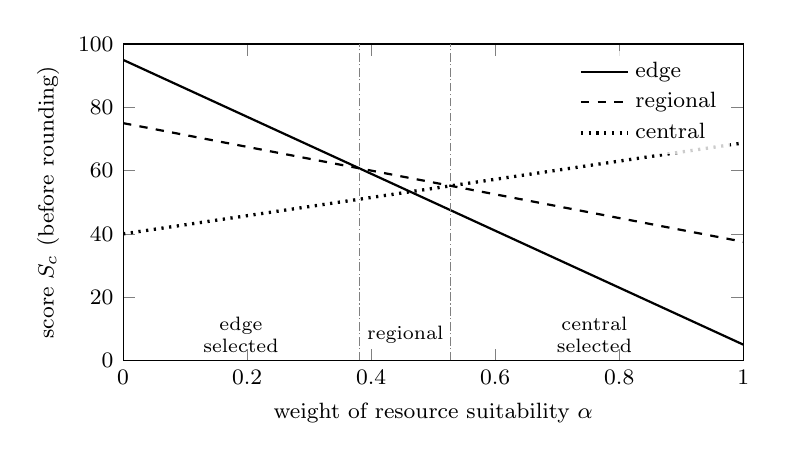
\begin{tikzpicture}
\begin{axis}[
  width=0.78\textwidth, height=5.6cm,
  xmin=0, xmax=1, ymin=0, ymax=100,
  xlabel={weight of resource suitability $\alpha$}, ylabel={score $S_c$ (before rounding)},
  xtick={0,0.2,0.4,0.6,0.8,1}, ytick={0,20,40,60,80,100},
  legend style={at={(0.98,0.98)}, anchor=north east, font=\footnotesize, draw=none, fill=white, fill opacity=0.8, text opacity=1},
  legend cell align=left,
  tick label style={font=\footnotesize}, label style={font=\footnotesize},
  every axis plot/.append style={thick, samples=2, domain=0:1},
]
\addplot[black, solid]        {100*(0.95 - 0.900*x)};  \addlegendentry{edge}
\addplot[black, dashed]       {100*(0.75 - 0.375*x)};  \addlegendentry{regional}
\addplot[black, dotted, very thick] {100*(0.40 + 0.2875*x)}; \addlegendentry{central}
\draw[gray, densely dashdotted] (axis cs:0.381,0) -- (axis cs:0.381,100);
\draw[gray, densely dashdotted] (axis cs:0.528,0) -- (axis cs:0.528,100);
\node[font=\scriptsize, align=center] at (axis cs:0.19,8) {edge\\selected};
\node[font=\scriptsize, align=center] at (axis cs:0.455,8) {regional};
\node[font=\scriptsize, align=center] at (axis cs:0.76,8) {central\\selected};
\end{axis}
\end{tikzpicture}
